\begin{figure}
    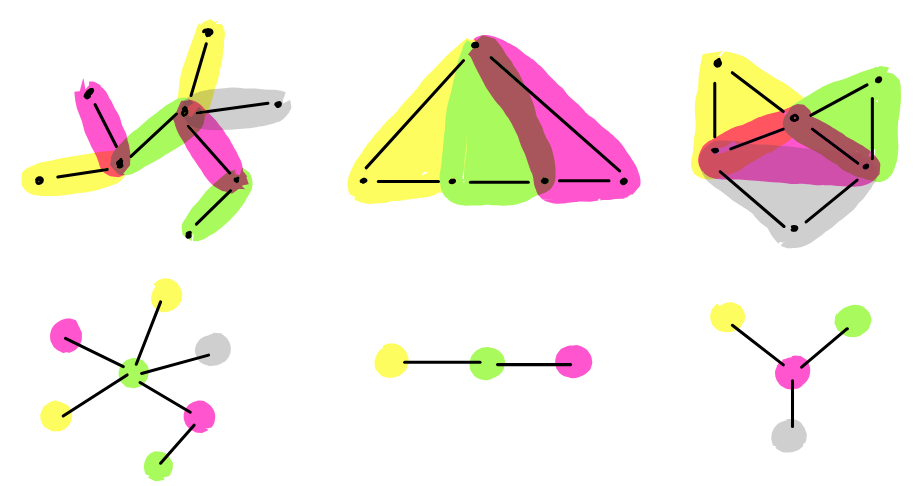
\includegraphics[width=\textwidth]{figures/treewidth-example.png}
    \caption{Examples of treewidth. (a) A tree has treewidth 1. (b) A cycle has treewidth 2. (c) A graph with treewidth 2. For each example, the bags of a tree decomposition of the graph is shown at the top, and the tree of the corresponding tree decomposition is depicted at the bottom.}
    \label{fig:treewidth-example}
\end{figure} 